\documentclass[11pt,a4paper]{article}

\usepackage[utf8]{inputenc}
\usepackage[T1]{fontenc}
\usepackage[spanish]{babel}
\usepackage[left=2cm,right=2cm,top=2cm,bottom=2cm]{geometry} % Márgenes 
\usepackage{url}
\usepackage{listings}
\usepackage{graphicx}

\lstdefinestyle{Python-color}{%
	language=Python,
	basicstyle=\scriptsize,
	otherkeywords={self},          
	keywordstyle=\bfseries\color{NavyBlue},
	emphstyle=\bfseries\color{DarkRed},    
	stringstyle=\color{ForestGreen}
}

\author{Antonio Manjavacas, Miguel Millán, Desiré Saponaro}

\title{\textbf{IMDb Data Warehouse} \\ Bases de Datos Avanzadas}

\date{\today}

\begin{document}

\maketitle

\begin{abstract}

Los almacenes de datos, también denominados \textit{Data Warehouses}, son bases de datos analíticas destinadas a la toma de decisiones así como a ofrecer perspectivas de alto nivel sobre las diferentes dimensiones de negocio. El principal objetivo de este trabajo es el desarrollo de un almacén de datos orientado al dominio de la industria cinematográfica, tomando como referencia los datos correspondientes a 5000 películas extraídos de \textit{IMDb} y ofrecidos por la plataforma \textit{Kaggle}.

\end{abstract}

\tableofcontents

\section{Introducción}

Definimos almacenes de datos (\textit{Data Warehouses}) como bases de datos analíticas, integradas, no volátiles y variables en el tiempo orientadas a la toma de decisiones en un determinado ámbito. Generalmente, los almacenes de datos reúnen una gran cantidad de información empleada desde la perspectiva de la analítica de datos y la ingeniería de negocio. Estos datos se encuentran orientados a temas y son fruto de la unión de múltiples subconjuntos de sistemas de información de más bajo nivel denominados \textit{Data marts}.

Una vez definido el concepto de \textit{Data Warehouse}, así como sus aplicaciones, el objetivo de este proyecto será llevar la elaboración de nuestro propio almacén de datos. El área de aplicación elegida ha sido la industria cinematográfica, empleando los datos proporcionados por la plataforma \textit{Kaggle} referentes a 5000 películas presentes en \textit{IMDb}. El conjunto de datos, así como una definición detallada del mismo, puede consultarse en el siguiente enlace: \url{https://www.kaggle.com/tmdb/tmdb-movie-metadata}.

Así, los resultados esperados tras el desarrollo de este proyecto incluirán tanto la limpieza, transformación y carga de datos en el sistema \textit{cloud} no relacional \textit{MongoDB Atlas}, como la elaboración de las diferentes dimensiones del almacén de datos.

Los principales medios tecnológicos empleados han sido: el entorno de programación Python, \textit{Google Colab}, orientado al desarrollo software colaborativo; \textit{MongoDB} y, concretamente, su servicio en la nube \textit{MongoDB Atlas}, para el almacenamiento de datos y \LaTeX para la elaboración de la memoria del proyecto.

\newpage
\section{Desarrollo}

En las siguientes subsecciones se detallará el proceso de elaboración de nuestro almacén de datos, desde el diseño del mismo hasta la limpieza y carga de los datos en sus diferentes dimensiones.

\subsection{Diseño y dimensiones del almacén de datos}

El esquema en estrella es un modelo de datos consistente en una tabla central (tabla de hechos) que contiene el conjunto de registros a analizar, así como una serie de tablas de dimensiones que la rodean. Dichas dimensiones ofrecen información más concreta y facilitan las labores de análisis sobre el conjunto de datos.

En este caso, el almacén de datos es una base de datos sobre películas, así que como tabla central tenemos la tabla con los datos de todas las películas de las que disponemos (Figura \ref{fig:almacen}).

\begin{figure}[h]
	\centering
	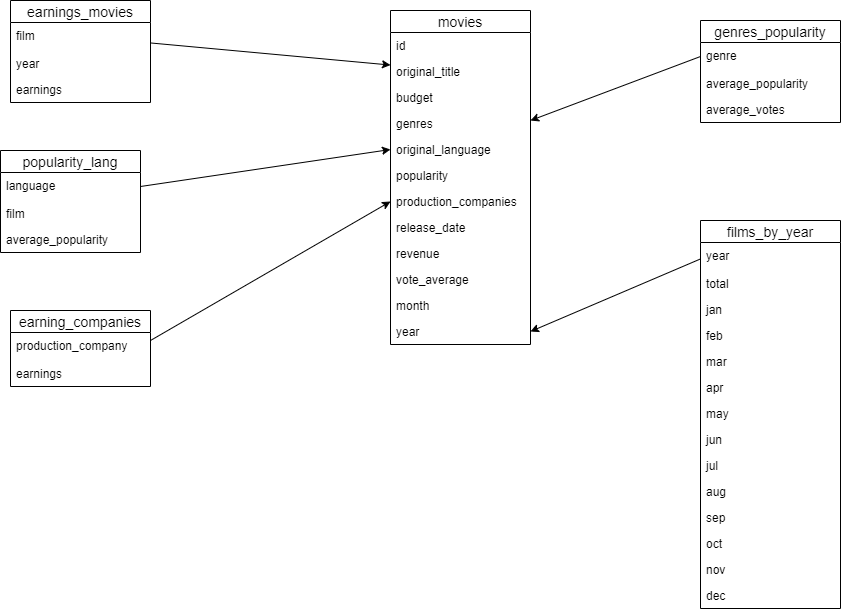
\includegraphics[width=0.9\linewidth]{./images/design.png} 
	\caption{Diseño del almacén de datos}
	\label{fig:almacen}
\end{figure}

Por otro lado, contamos con las siguientes dimensiones:

\begin{itemize}
	\item \textbf{Dimensión 1}. La primera dimensión está compuesta por las películas que más dinero generaron por año, calculada basándonos en la diferencia entre presupuesto de la película y las ganancias totales. Véase la Figura \ref{fig:dim1}.
	
	\begin{figure}[h]
		\centering
		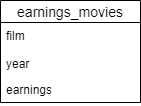
\includegraphics[width=0.2\linewidth]{./images/Dimension1.png} 
		\caption{Dimensión earnings\_movies}
		\label{fig:dim1}
	\end{figure}
	
	\item \textbf{Dimensión 2}. Muestra la película más popular para cada idioma. Las consultas a esta tabla pueden ser de utilidad para estudiar que tipo de película gusta más en función del idioma que hablan los espectadores. Véase la Figura \ref{fig:dim2}.
	
	\begin{figure}[h]
		\centering
		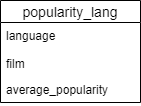
\includegraphics[width=0.2\linewidth]{./images/Dimension2.png} 
		\caption{Dimensión popularity\_lang}
		\label{fig:dim2}
	\end{figure}
	
	\item \textbf{Dimensión 3}. Representa las ganancias totales de las diferentes compañías productoras. Estos datos permiten conocer qué productoras han generado mayores beneficios. Véase la Figura \ref{fig:dim3}.
	
	\begin{figure}[h]
		\centering
		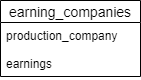
\includegraphics[width=0.2\linewidth]{./images/Dimension3.png} 
		\caption{Dimensión earning\_companies}
		\label{fig:dim3}
	\end{figure}
	
	\item \textbf{Dimensión 4}. Compuesta por la popularidad y nota medias entre las películas de cada género. Con dicha información es posible conocer que géneros atraen más al público. Véase la Figura \ref{fig:dim4}.
	
	\begin{figure}[h]
		\centering
		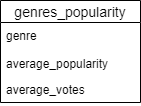
\includegraphics[width=0.2\linewidth]{./images/Dimension4.png} 
		\caption{Dimensión genres\_popularity}
		\label{fig:dim4}
	\end{figure}
	
	\item \textbf{Dimensión 5}. Muestra el número de películas realizadas por año, además del número de películas por mes dentro de dicho año. Su utilidad reside en poder conocer en qué año se estrenaron más películas o en qué suelen producirse más estrenos. Véase la Figura \ref{fig:dim5}.
	
	\begin{figure}[h]
		\centering
		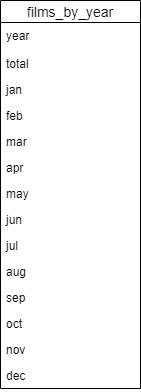
\includegraphics[width=0.2\linewidth]{./images/Dimension5.png} 
		\caption{Dimensión films\_by\_year}
		\label{fig:dim5}
	\end{figure}
	
\end{itemize}

\subsection{Limpieza y carga de datos}

Una vez definido el diseño y dimensiones de nuestro \textit{Data Warehouse}, procedemos a explicar cómo se llevó a cabo la limpieza y transformación del conjunto de datos inicial de cara a su posterior carga en \textit{MongoDB Atlas}. Las diferentes labores del proceso de \textit{data cleaning} se definen en los siguientes puntos:

\begin{itemize}
\item \textbf{Extracción de las características de interés}. Las columnas extraídas del conjunto de datos original fueron:

	\begin{itemize}
	\item Identificador de la película.
	\item Título original.
	\item Presupuesto.
	\item Géneros.
	\item Idioma original.
	\item Popularidad.
	\item Compañías productoras.
	\item Fecha de lanzamiento.
	\item Ganancias.
	\item Puntuación media.
	\end{itemize}

\item \textbf{Eliminación de registros con valores nulos}. Se decidió optar por la eliminación de aquellas películas con información incompleta, ya que podrían perjudicar a los resultados finales.

\item \textbf{Conversión del formato de la columna \textit{géneros}}. Se modificó el formato de esta columna, inicialmente expresada como JSON, y se convirtió en una lista de géneros, eliminando su identificador.

\item \textbf{Conversión del formato de la columna \textit{compañías productoras}}. El procedimiento fue similar al caso anterior: se eliminaron identificadores y las compañías productoras quedaron expresadas como listas.

\item \textbf{Conversión del formato de las fechas de lanzamiento}. Las fechas, inicialmente expresadas en formato AA/MM/DD, fueron convertidas al formato DD/MM/AA.

\item \textbf{Creación de las columnas \textit{month} y \textit{year}}. Estas columnas facilitarían el trabajo en la elaboración de la mayoría de las dimensiones.

\end{itemize}

Una vez procesados los datos, contamos con un total de 4802 registros que fueron cargados en la base de datos.

\section{Resultados y conclusiones}

Una vez las diferentes dimensiones fueron cargadas en la base de datos, se procedió a la recuperación de información ya ubicada en la base de datos en la nube. Los resultados correspondientes a dichas consultas son los que se muestran en las Figuras \ref{fig:query1}, \ref{fig:query2}, \ref{fig:query3}, \ref{fig:query4} y \ref{fig:query5}.

	\begin{figure}
		\centering
		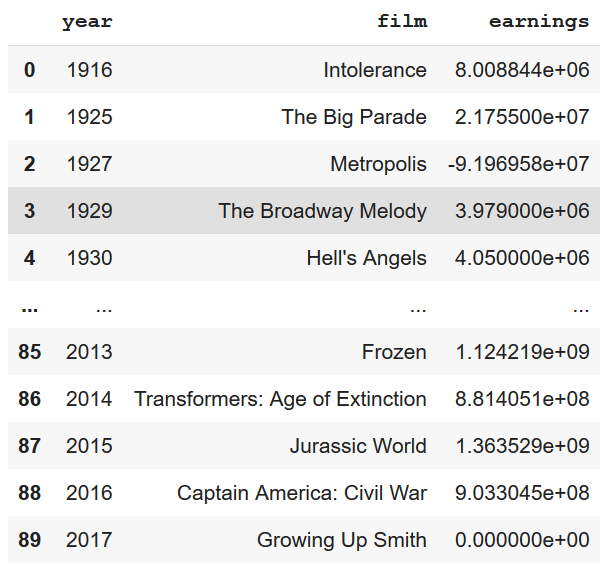
\includegraphics[width=0.6\linewidth]{./images/query1.png} 
		\caption{Consulta a la base de datos: dimensión \textit{earnings movies}}
		\label{fig:query1}
	\end{figure}

	\begin{figure}
		\centering
		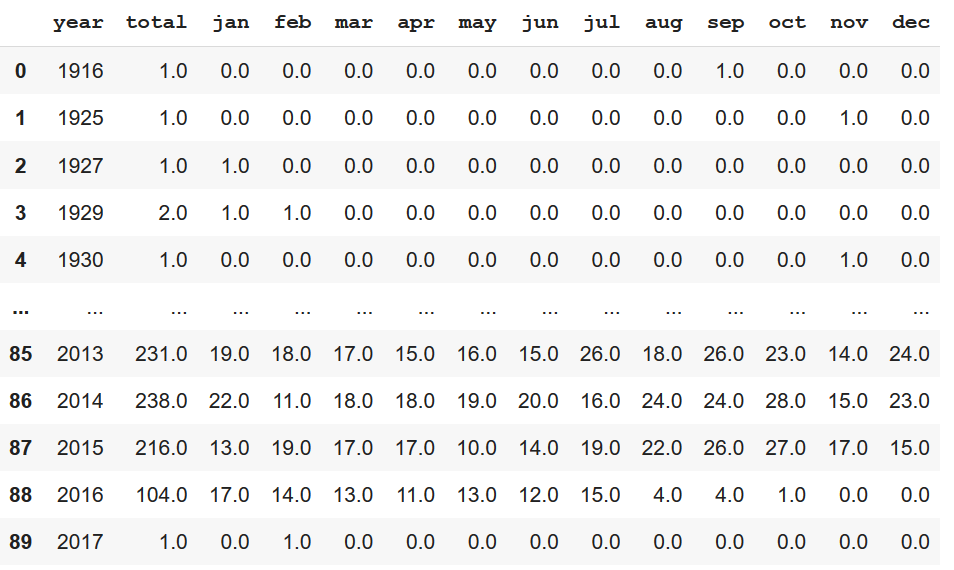
\includegraphics[width=0.6\linewidth]{./images/query2.png} 
		\caption{Consulta a la base de datos: dimensión \textit{films by year}}
		\label{fig:query2}
	\end{figure}
	
	\begin{figure}
		\centering
		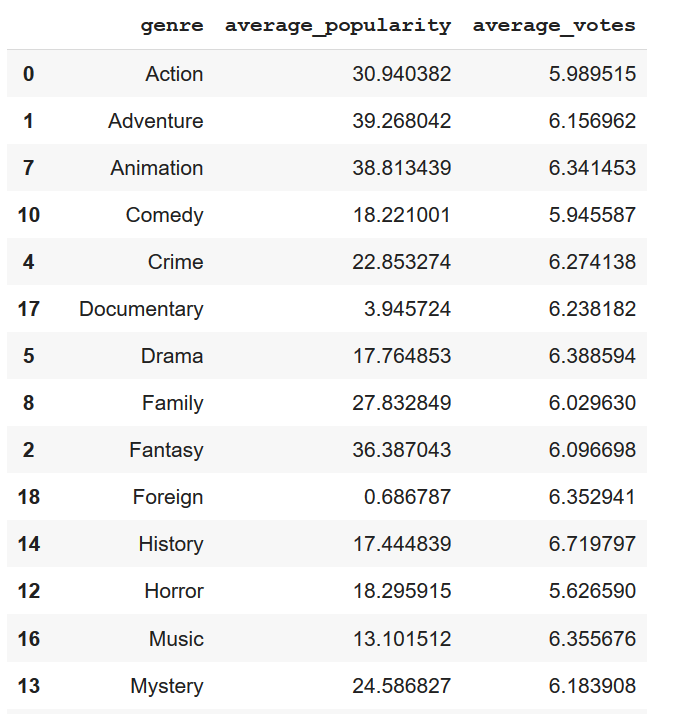
\includegraphics[width=0.6\linewidth]{./images/query3.png} 
		\caption{Consulta a la base de datos: dimensión \textit{genres popularity}}
		\label{fig:query3}
	\end{figure}

	\begin{figure}
		\centering
		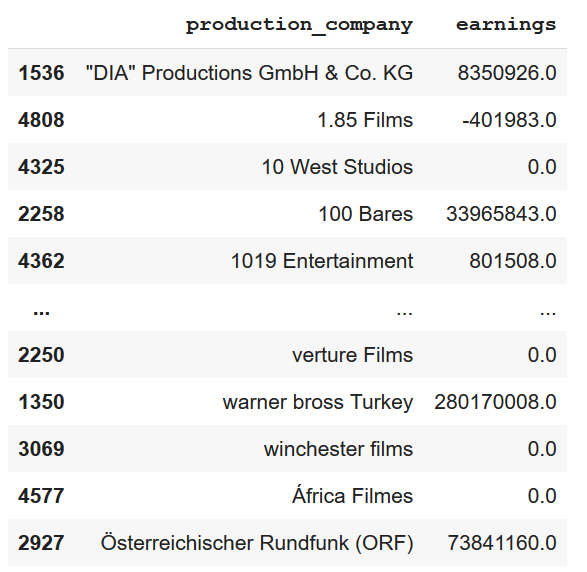
\includegraphics[width=0.6\linewidth]{./images/query4.png} 
		\caption{Consulta a la base de datos: dimensión \textit{earnings companies}}
		\label{fig:query4}
	\end{figure}
		
	\begin{figure}
		\centering
		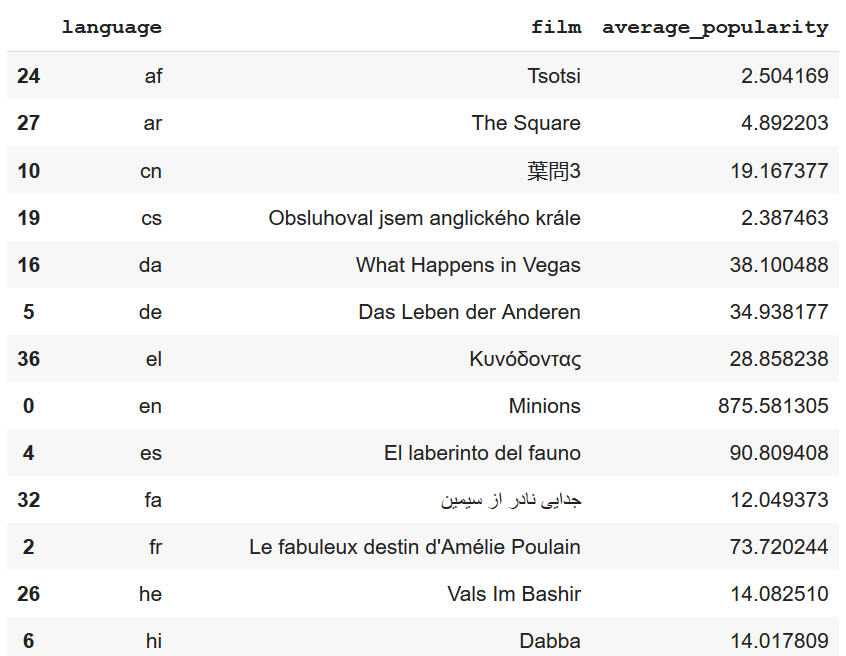
\includegraphics[width=0.6\linewidth]{./images/query5.png} 
		\caption{Consulta a la base de datos: dimensión \textit{popularity lang}}
		\label{fig:query5}
	\end{figure}
	
Los resultados de este proyecto han sido satisfactorios y nos han permitido comprender el proceso ETL (extracción, transformación y carga de datos) de un almacén de datos de forma práctica. Toda la información referente al código empleado puede consultarse en \url{https://github.com/manjavacas/BBDD-Avanzadas}.

\end{document}